% \chapter{Objectives}
\section{Thesis statement}
\subsection{Thesis statement}\label{thesis-statement}
Several solutions has been proposed to deal with the routing problem in wireless sensor network with holes \cite{gpsr,boundhole,ehds,elbar,ellipse,issnip}. The most well-known solution is the Greedy Perimeter Stateless Routing (\emph{GPSR}) protocol, which was proposed by B.Karp in 2000 \cite{gpsr}. This algorithm computes a planar graph for the network in which its vertices are sensor nodes and its edges are edges connecting sensor nodes and its neighbors. The packet is then forwarded based on edges of the graph. In 2005, Qing Fang and her colleagues proposed a novel algorithm (the BOUNDHOLE algorithm) to detect the boundary of the routing hole \cite{boundhole}. In addition, these authors also proposed a routing protocol based on the determined hole boundary: when the packet reaches a \emph{stuck node}\footnote{A stuck node is a node where a packet may get stuck and is more likely to occur the local minimum phenomenon. We will discuss further more about stuck node definition in section \ref{chapter3.1-boundhole}.} \emph{S}, it is forwarded along the boundary of the hole until it reaches an intermediate sensor node that is closer to the destination node than \emph{S}. 

Other solutions based on the BOUNDHOLE algorithm has also been proposed. The common idea is that these protocols construct a forbidden area covering the hole and broadcast the information of this area to the network. The source node then uses these information to calculate the routing path. The forbidden area is usually a simpler shape such as circle \cite{ehds}, ellipse \cite{ellipse}, parallelogram \cite{elbar}, or octagon \cite{issnip}. In \cite{issnip}, the authors also proposed a non-trivial approach that is to use some random factors to ensure mentioned requirements of routing in wireless sensor network such as load balancing, energy efficiency and route stretch.

\begin{figure}[!htb]
\centering
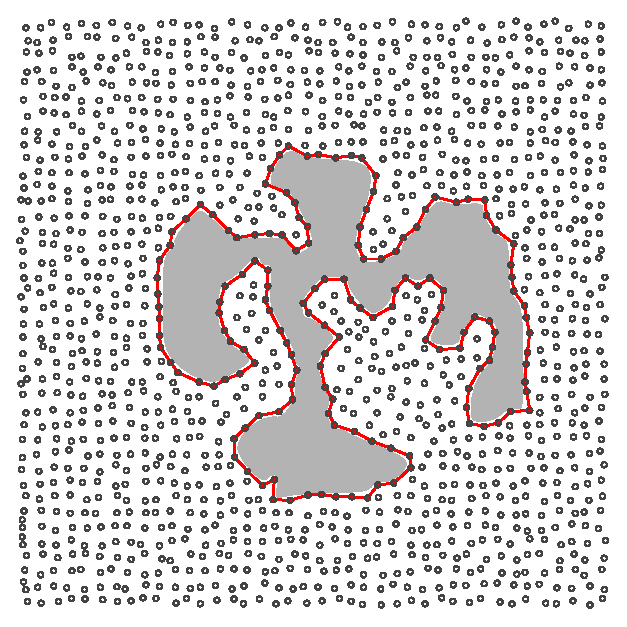
\includegraphics[width=0.4\textwidth]{Chapter2/Chapter2Figs/fig-polygon.eps}
\caption{An example of hole polygon.}
\centering
\small {In this figure, the gray region is the hole and the red line is the hole boundary.}
\label{cave-regions}
\end{figure}

However, the routing hole in wireless sensor network can be a random, complex shape and thus, may have a lot of cave regions. Figure \ref{cave-regions} shows an example of hole shape. \emph{Near hole routing} problem is defined as a problem to find the routing path in which the source node or the destination node, or both of them lie nearly the hole, in the boundary of the hole or inside the cave areas. The difficulty of this problem probably is to construct a path for packet to route out the hole when the source node is inside a cave or to construct a path to forward packet from outside to a destination which is inside a cave. Most of the above algorithms have been ignored the near hole routing problem. In such a case, they all use the GPSR algorithm to compute the routing path. This generally degrades the efficiency of these protocols in case there requires a lot of near hole routings. This leads to the necessity of a good \emph{near hole routing protocol} to fulfill requirements of routing in wireless sensor networks.

\subsection{Objectives}
Based on the described problem in subsection \ref{thesis-statement}, the objectives of my thesis are:
\begin{enumerate}
\item \emph{Study related works about geographical routing in wireless sensor network with holes.} We need to make a survey about previous works: their advantages and disadvantages. Generally, a routing protocol consists of two phases: the initial phase when the network learns about the hole shape and computes parameters of the protocol and the data forwarding phase when the network starts sending data packets. Most of previous works use different shapes to approximate the hole polygon in the initial phase. Thus, it is supposed to analyze these shapes to find out the most appropriate shape for the hole approximation since the approximate hole impacts the load balancing, routing stretch and hence, network's energy consumption.
\item \emph{Propose a solution for the near hole routing problem.} Currently, as our knowledge, there are no protocols that can deal with the near hole routing problem except GPSR and BOUNDHOLE. We will propose a protocol which targets to achieve both two main requirements of routing in wireless sensor network with holes, that is load balancing and energy consumption. This is also the main objective of my thesis.
\item \emph{Modify the BK-WisSim toolkit to adapt more requirements of network simulation.} \emph{BK-WisSim} is a visual network simulation tool developed by SEDIC Lab \cite{wissim-web}. We continue developing this tool to support more requirements of network simulation, such as improving the current Energy Model of \emph{ns-2} and developing new features for \emph{BK-WisSim}.
\item \emph{Implement proposed protocol and do experimental evaluations to compare it with current protocols.} The last mission is implementing proposed protocol and embedding it into the core of \emph{BK-WisSim}. Then the proposed protocol will be compared with current exist protocols (GPSR, BOUNDHOLE) to evaluate its performance and proof that it totally satisfies the requirements.
\end{enumerate}

\subsection{Results and Contributions}
\paragraph{Studied related works about geographical routing in wireless sensor network with holes. \\}
We have provided a survey about previous works. In this survey, firstly, we described the BOUNDHOLE algorithm and explained the reason why we need to use this algorithm to detect the routing hole instead of other algorithms; secondly, we described an overview about each protocol and pointed out their pros and cons. We have also come up a conclusion that octagon is the most appropriate shape to use to approximate the hole based on theoretical analyses given by its authors.

\paragraph{Proposed the near hole routing protocol.\\}
This algorithm is my primary research, conducted from studies and research to find a solution for near hole routing problem. This algorithm solves the difficulty of the near hole routing problem by constructing the Voronoi diagram \cite{voronoi} of the hole polygon and then creating a graph which is a \emph{``skeleton''} of this polygon based on the Voronoi diagram. This graph is used to make the routing path for the packet to get out or get in the cave. It also inherits the previous result, that is using octagon to approximate the hole in initial phase and using random factors in routing phase. We also provided some theoretical analyses to prove the validity of the protocol, a discussion about the impact of protocol's parameters. This proposed algorithm not only inherits the advantages of previous algorithm but also completely solves the near hole routing problem.

\paragraph{Updated BK-WisSim toolkit.\\}
We have improved the Energy Model of \emph{ns-2} to support more experimental scenarios and to extract more information about the simulation process. We also developed some new feature for \emph{BK-WisSim} client including: supporting graph algorithms (Voronoi diagram and Dijsktra algorithm) in WisSim Editor, simulating the simulation process via animation in WisSim Visualizer and more. 

\paragraph{Evaluation of proposed protocol.\\}
We proposed some evaluation metrics and scenarios for experiments. These metrics are: energy consumption, deviation of energy consumption, load balancing, routing path length and network lifetime. The experiments were performed to compare the proposed protocol with GPSR and BOUNDHOLE algorithm. The results shown that our proposed protocol is better than both the other algorithms in all evaluation metrics. We also performed some specific experiments for our proposed protocol to analyze the impact of protocol's parameters on energy consumption and routing stretch.

The remainder of this thesis is organized as follows. In chapter \ref{chapter3}, we discuss about the BOUNDHOLE algorithm and related works. The details of proposed protocol is presented in chapter \ref{chapter4}. In this chapter, we firstly describe the protocol details and then provide some theoretical analysis of proposed protocol. In chapter \ref{chapter5}, we give an overview about \emph{ns-2} and \emph{BK-WisSim} toolkit. We also introduce new features of \emph{BK-WisSim} in this chapter. The source code and detailed implementation of proposed protocol is provided in chapter \ref{chapter6}. In chapter \ref{chapter7}, we present the simulation result to evaluate the performance of the protocol. Finally, we conclude the thesis in chapter \ref{chapter8}. 